\section{Reproduzierbarkeit und Projektartefakte}

\subsection{Zentrale Implementierungen}

\begin{itemize}
    \item \textbf{Cross-Validation-Splits:}\\ \texttt{mmdetection3d/tools/dataset\_converters/}\\\texttt{create\_exp\_crossval\_splits.py}
    \item \textbf{PointPillars-CV-Konfiguration:}\\ \texttt{mmdetection3d/configs/pointpillars/}\\\texttt{pointpillars\_hv\_secfpn\_8xb6-50e\_exp-crossval-gtsample.py}
    \item \textbf{Trainingssteuerung:}\\ \texttt{mmdetection3d/tools/run\_exp\_crossval.sh}
    \item \textbf{Cross-Validation-Auswertung:}\\ \texttt{mmdetection3d/tools/analysis\_tools/exp\_eval\_crossval.py}
    \item \textbf{Geisterboxanalyse:}\\ \texttt{mmdetection3d/tools/analysis\_tools/exp\_ghost\_boxes\_crossval.py}
    \item \textbf{Punktwolken-Merge:} \texttt{experiment/pcd\_merge.py}
    \item \textbf{Label-Editor:} \texttt{experiment/manual\_bbox\_editor.py}
\end{itemize}

\subsection{Primäre Ergebnisquellen}

\begin{itemize}\raggedright
    \item \texttt{results/CROSS\_VALIDATION.md}: eingefrorenes Evaluationsprotokoll
    \item \texttt{results/CROSS\_VALIDATION\_RESULTS.md}: offizielle PointPillars-Ergebnisse
    \item \texttt{results/CROSS\_VALIDATION\_STATIC\_AWARE.md}: labelbasierte Teilbewertung
    \item \texttt{results/CENTERPOINT\_CV\_STATIC\_AWARE.md}: CenterPoint-Vergleich
    \item \texttt{results/GHOST\_BOXES.json}: generalisierte OOF-Fehlerzählung
    \item \texttt{results/DATA\_AUDIT.md}: Daten-, Metrik- und Ursachenanalyse
    \item \texttt{results/ABLATION\_BICYCLE.md}: frühere kontrollierte Ablationen
\end{itemize}

\subsection{Präsentationsmaterial}

Das primäre qualitative Video ist \texttt{results/videos/}\\\texttt{exp1\_cv\_full\_three\_views\_oblique.mp4}. Es zeigt alle 105 gemeinsamen gültigen Frames von Experiment 1 mit den drei Fold-1-Modellen, für die das vollständige Experiment während Training und Checkpoint-Auswahl ungesehen war. Abbildung~\ref{fig:drei-sichten} zeigt ein Standbild daraus.

\begin{figure}[H]
\centering
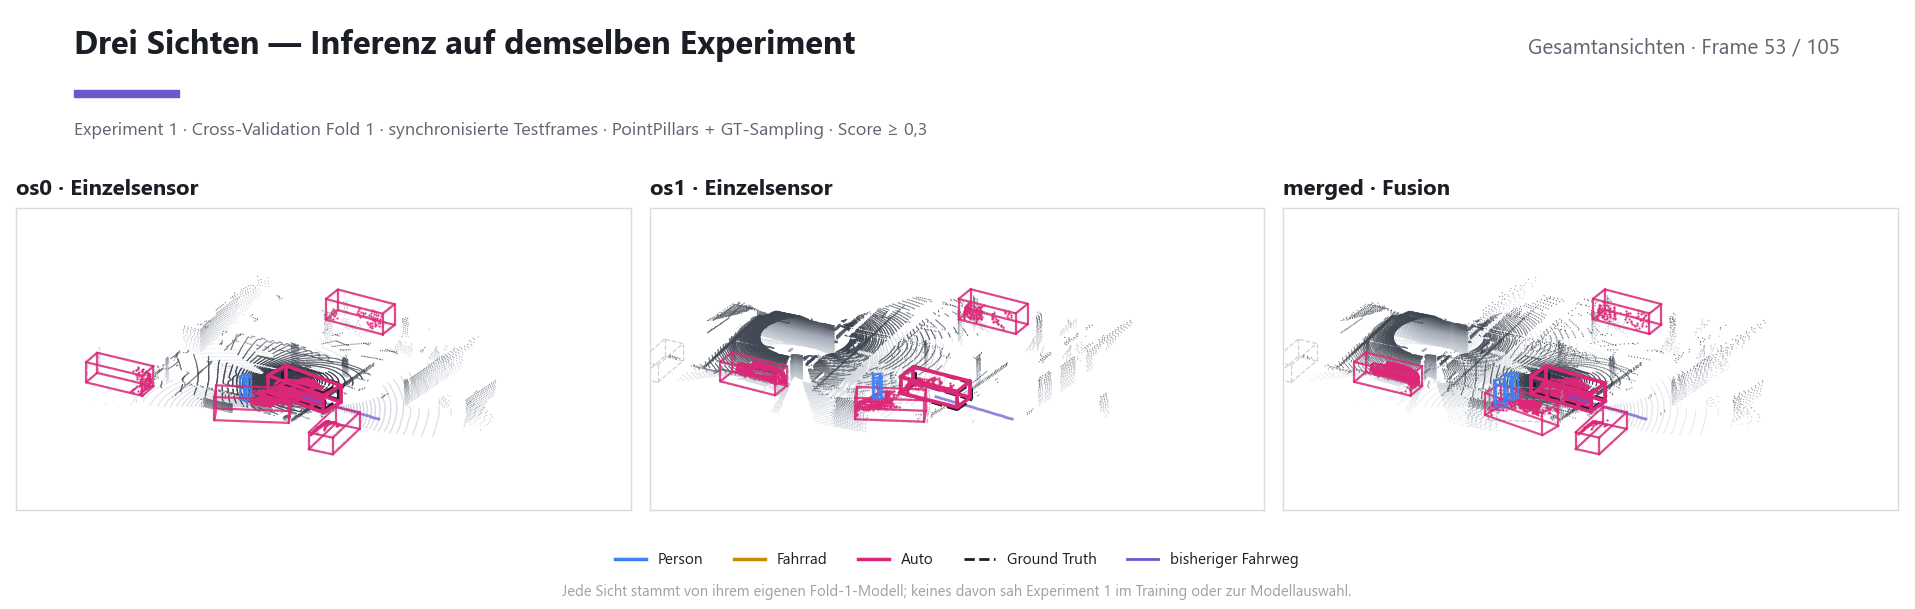
\includegraphics[width=\textwidth]{images/drei-sichten-standbild.png}
\caption{Standbild aus dem qualitativen Video: dieselbe Szene aus \texttt{os0}, \texttt{os1} und \texttt{merged}, jeweils vorhergesagt vom zugehörigen Fold-1-Modell.}
\label{fig:drei-sichten}
\end{figure}

Ältere Videos des temporalen 11-Frame-Testsegments sind nur historische Artefakte. Sie dürfen nicht als Beleg dafür verwendet werden, dass \texttt{os1} das bewegte Auto generell nicht erkennen könne.
